\documentclass[a4paper, 12pt, oneside, table]{article}
\usepackage[square, numbers, comma, sort&compress]{natbib}  % Use the "Natbib" style for the references in the Bibliography
\usepackage{verbatim} 
\usepackage[english]{babel}
\usepackage[utf8]{inputenc}
\usepackage{graphicx}
\usepackage{multirow}
\usepackage{amsmath}
\usepackage{amssymb}


%\usepackage{cite}
\usepackage{booktabs}
\usepackage{listings}
\usepackage{epstopdf}
\usepackage{helvet} 
\renewcommand{\familydefault}{\sfdefault}
\usepackage{setspace}
\singlespacing % interlinea singola
\linespread{0.97}
\usepackage{color}
\usepackage[margin=2.5cm]{geometry}
\setlength{\parindent}{0pt}
% pacchetti aggiunti
\usepackage{comment}
\usepackage[export]{adjustbox}
\usepackage{subfigure}
%\usepackage{subcaption}
\usepackage{algorithm}
\usepackage{algorithmic}
\usepackage{amsfonts}
\usepackage{tabularx}
\usepackage{ltablex}
\usepackage{caption}
\usepackage{titling}
\usepackage{spreadtab}
\renewcommand\maketitlehooka{\null\mbox{}\vfill}
\renewcommand\maketitlehookd{\vfill\null}

\usepackage{comment}

\usepackage{mathtools}
\DeclarePairedDelimiter{\floor}{\lfloor}{\rfloor}

\usepackage{enumerate}
\usepackage{enumitem}
\usepackage[dvipsnames]{xcolor}
\newcommand*{\lorenzo}[1]{\textcolor{BurntOrange}{#1}}
\newcommand{\yasmin}[1]{\textcolor{Red}{#1}}
\newcommand{\giovanni}[1]{\textcolor{Blue}{#1}}


\title{RASD}
\author{Yasmin Awad, Lorenzo Carpaneto, Giovanni Dispoto}
\date{November 2020}

\begin{document}

\begin{titlepage}
%\vspace*{\fill}
\begin{figure}[h!]
	\centering
	
\includegraphics[scale=0.5]{img/logopoli.png}
\end{figure}
\vspace{0.7em}
\begin{center}
	\Large \textbf{DD}
\end{center}
%\begin{center}
%	\large Version 0.1
%\end{center}
%\begin{center}
%	\large Version Date
%\end{center}
%\vspace{0.4em}
\begin{center}
	\Large \textbf{CLup – Customers Line-up } 
\end{center}
\vspace{-0.6em}
\begin{center}
	\normalsize Yasmin Awad, Lorenzo Carpaneto, Giovanni Dispoto
	\begin{figure}[h!]
	\centering
	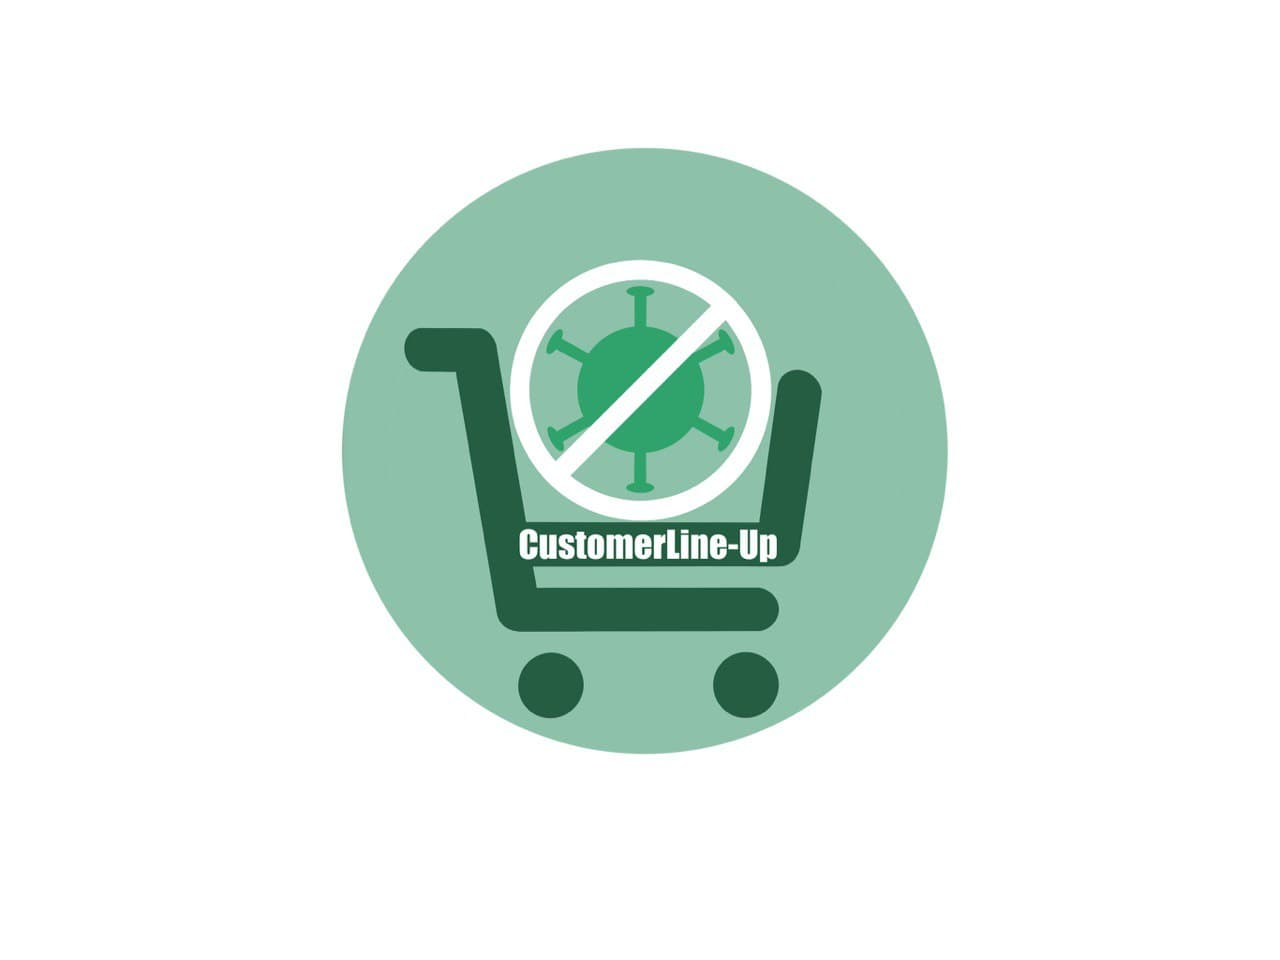
\includegraphics[scale=0.25]{img/logo.jpg}
\end{figure}
\end{center}
\vspace*{\fill}
\end{titlepage}

\normalsize


\newpage
\tableofcontents
\newpage

\section{Introduction}
\subsection{Purpose}
After showing a general description of the CL-up application within the RASD, this document focuses on analyzing the system's architecture and design, in order to satisfy the various requirements stated in the previous document. The purpose of the document is to provide a functional description of the main architectural components, showing their runtime behaviour and interactions and their interfaces. This document is mainly intended to be used by the developers and testers.

\subsection{Scope}
Customer Line-up (CL-up) is an application that aims to allow accesses to Stores in a safe way. The objective is to avoid as much as possible queue formation outside the Stores and limits the number of people inside it in an efficient way. To pursue this goal, the application allows Users to register either as a Managers or Customers, providing services to both of them. Managers can create their Stores within the app and allow other Managers to help them in the organization of the Store rules. Tools are provided to allow Customers to book Visits or Tickets to the Stores remotely, allowing a greater and more efficient way for maintaining social distancing. This is done by the use of a virtual queue managed by the System, in which Customers' Reservations are stored and managed. In order to organize the various entrances in the Stores, an identifier for each Consumer will be used, that is a QRCode.\\ %The application provides also a fall-back option (Paper Tickets) and suggestions for Customers.
\\
More information can be found in the Chapter 1 of the RASD.

\newpage
\section{Architectural Design}
\subsection{Overview: High-level components and their interaction}
In this chapter the architectural structure of the System will be described. In Figure \ref{high_level_overview_img} the high level overview of the System is shown. In the next sections we will describe in detail the various components and their interactions.

\begin{figure}[h!]
\centering
	\centering
  	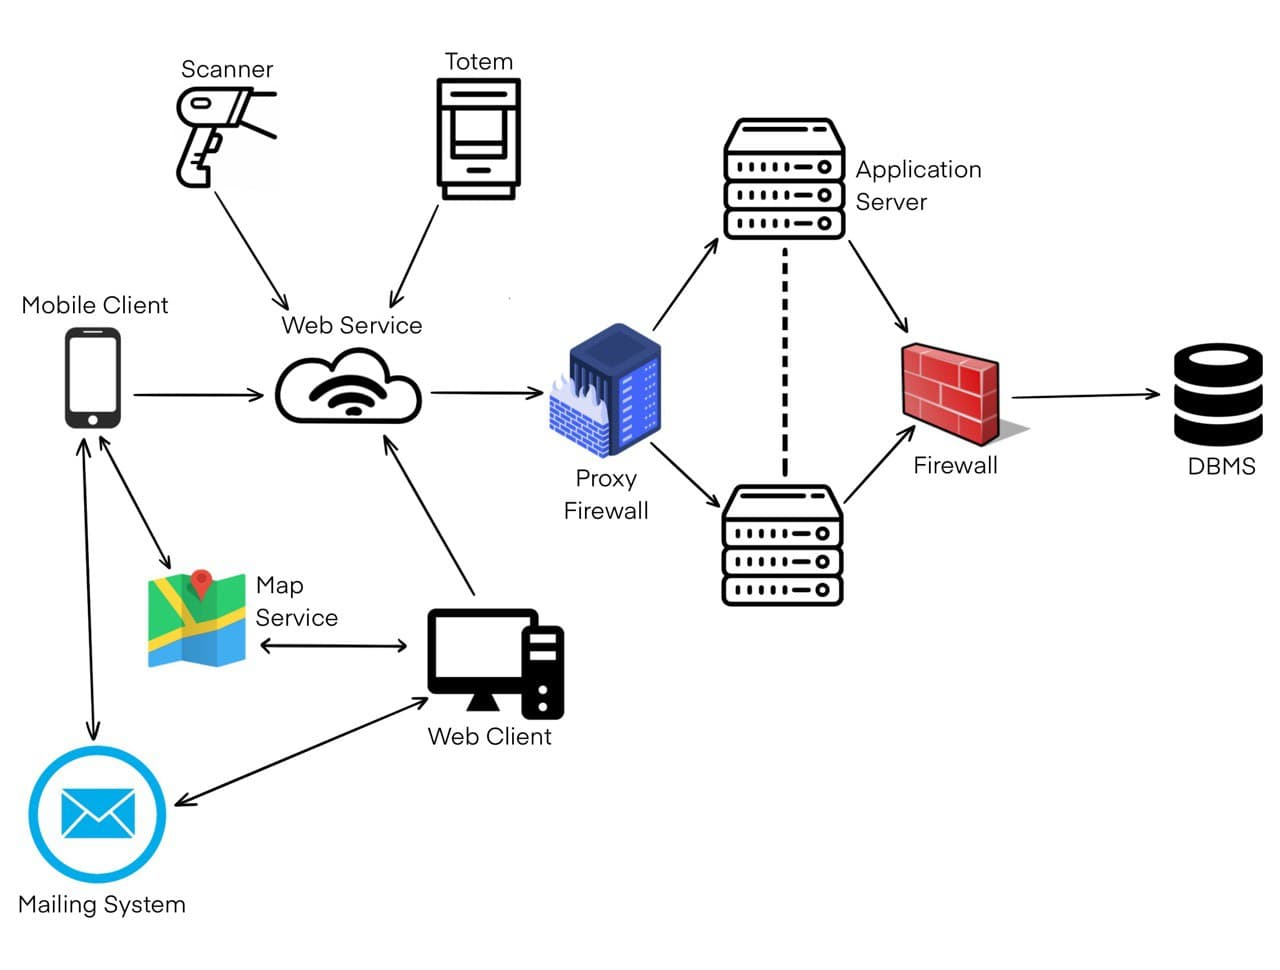
\includegraphics[height=0.4\textheight, scale=0.3, keepaspectratio]{img/high_level_overview.jpg}
	\caption{High-level overview of the System.}
 	\label{high_level_overview_img}
\end{figure}

\subsection{Component View}
To describe the internal modular structure of the components, we show how they are connected together in the UML component diagram in Figure \ref{comp_view_img} Components are wired together using an \textit{assembly connector} to connect the required interfave of one component with the provided interface of another component.

\begin{figure}[hbt]
\centering
	\centering
  	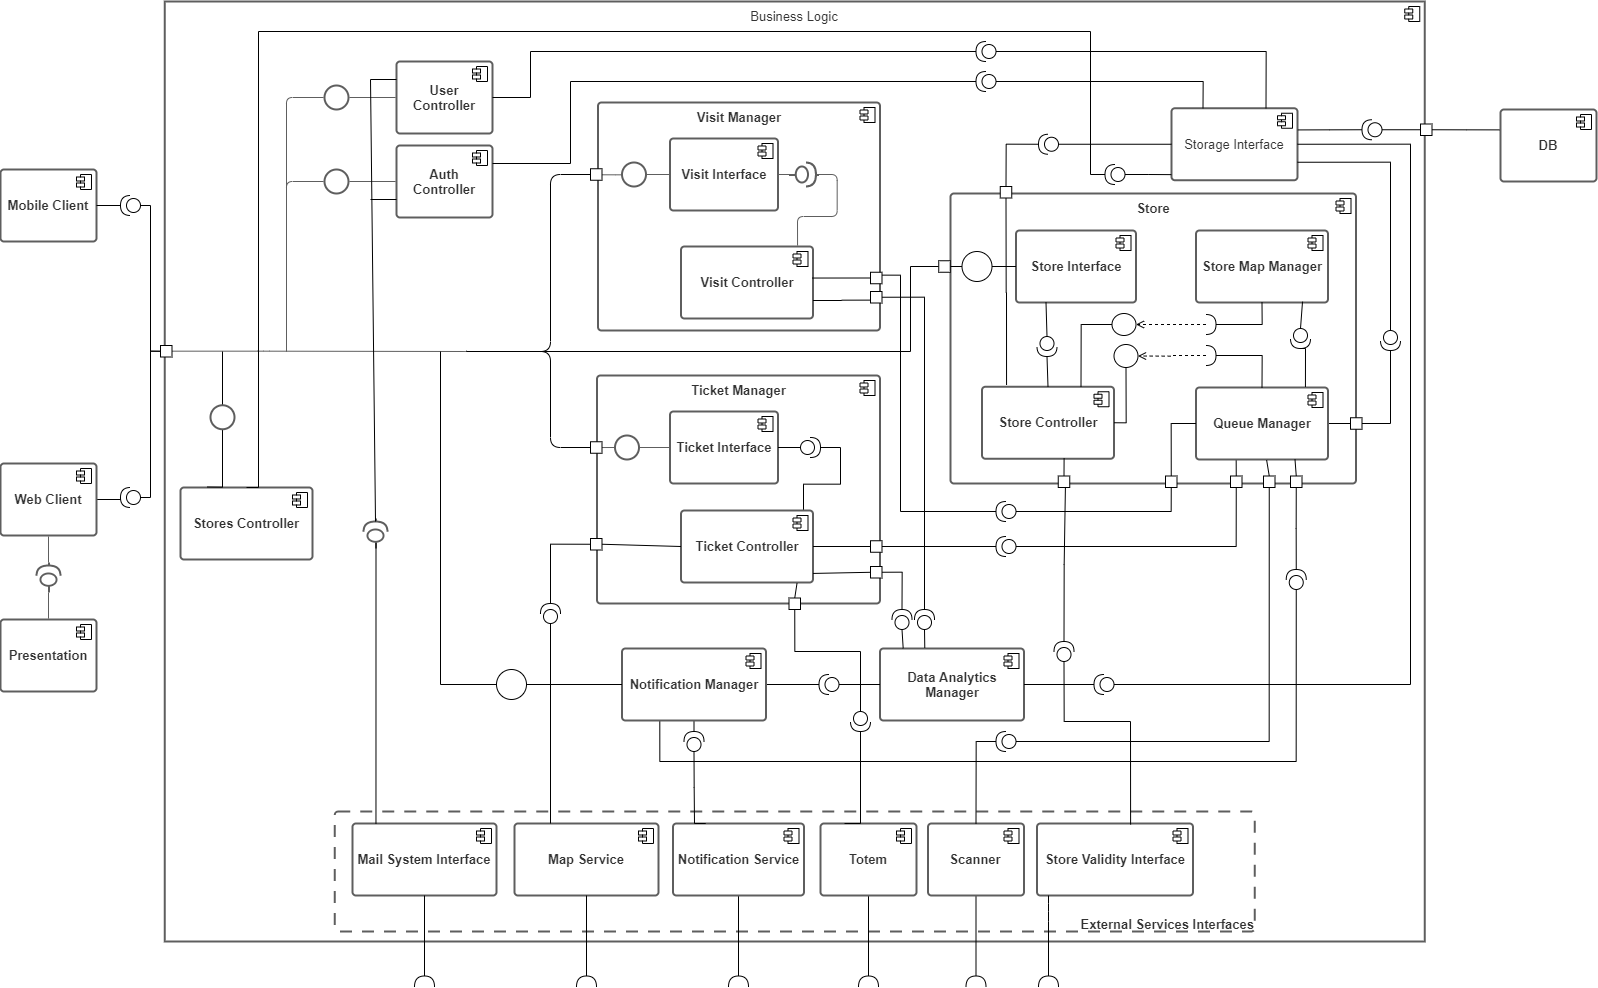
\includegraphics[height=0.4\textheight, scale=0.2, keepaspectratio]{img/component_view.png}
	\caption{Component diagram of the system.}
 	\label{comp_view_img}
\end{figure}

\begin{itemize}
    \item \label{cv:client}\textbf{Mobile Client} and \textbf{Web Client}: represents the two machines that accesses the entire System and it's functionalities. They both do not have important functions on their own, because we chose to implement them using a Thin Client approach.
    \item \textbf{Presentation}: it is used in order to display web pages of the application to a Web Client accessing through the browser. This layer only provides the structure of the user interface without accessing any data or application logic \lorenzo{forse metterei solo non accede all'application logic, perche' ai dati in qualche modo deve accederci per farli visualizzare su schermo (anche se puo' non sapere come siano stati estrapolati)}.
    \item \textbf{User Controller}: This component handles all the operations that affects the user data. It exposes method to change account credentials and stores them in the database.
    \item \textbf{Auth Controller}: This component handles all the operation for the authentication such as registration process and login process. It communicate with DBMS through Storage Interface in order to retrieve and insert user credentials. During the registration process or change password this component use Mailing System Interface
    \item \textbf{Data Analytics Manager}: is a component used in order to analyze Customers habits. In practice is a Recommender System that takes care of showing to a Customer the Stores most appealing to him and the best duration value to be included in a Reservation.
    \item \textbf{Notification Manger}: is a component used in order to provide Notifications to the Customer, such as  Virtual Tickets departures, appealing time slots of specific Stores and suggestions.
    \item \textbf{Ticket Manager}: is a subsystem component in charge of managing Ticket requests:
    \begin{itemize}
        \item \textbf{Ticket Interface}: it exposes to the Customer an Interface for compiling the requested Ticket attributes.
        \item \textbf{Ticket Controller}: it checks the validity of the inserted Ticket's attributes requested. Moreover it communicates with the Queue Manager in order to verify the possibility to accomplish the request.
    \end{itemize}
    \item \textbf{Visit Manager}:is a subsystem component in charge of managing Visit requests:
    \begin{itemize}
        \item \textbf{Visit Interface}: it exposes to the Customer an Interface for compiling the requested Visit attributes.
        \item \textbf{Visit Controller}: it checks the validity of the inserted Visit's attributes requested. Moreover it communicates with the Queue Manager in order to verify the possibility to accomplish the request.
    \end{itemize}
    \item \textbf{DB}: it represents the DBMS, which provide an interface to read and store data. User credentials, Stores information and queues reservations are stored  in the database.
    \item \textbf{Storage Interface}: it provide methods to access to database. This interface is needed in order to decouple all the components from the DBMS technology.
    \item \textbf{Store}: is a subsystem component in charge of managing Store and its Queue:
    \begin{itemize}
        \item \textbf{Store Interface}: it exposes to the Manager an Interface for creating and managing Stores.
        \item \textbf{Store Controller}: it ensures that a Manager intending to become Owner of a Store within the application has the necessary authorizations, checking the validity of the information by acquiring specific credentials. \yasmin{dovrei collegarlo a un external service di verifica??}
        \item \textbf{Queue Manager}: this component receives requests for Reservations for the Store, checks that they can be placed in the queue and eventually inserts them. It communicates with the Ticket Controller, the Visit Controller, the Scanner and the Totem. It also communicate with the DB in order to retrieve and modify all the necessary information.
        \item \label{comp:storeMapMan} \textbf{Store Map Manager}: this component receives requests from the Customers who has already booked a Visit. It has to populate the map with the path that the Customer should follow during their Visit inside the Store. It communicates with the Queue Manager to look at the specified departments by other people during the time-slot of the Visit specified.
    \end{itemize}
    \item \textbf{External Services Interfaces}: this set of components have as main objective to make API calls to the necessary third party services:
    \begin{itemize}
        \item \textbf{Mailing System Interface}: is an interface in charge of sending confirmation mails at the end of the registration process to the User. It also can send other type of notification mails.
        \item \textbf{Map Service}: this service is used in order to retrieve the necessary information about a Customer position. This information is used by the Data Analytics System and by the Ticket Controller \yasmin{???? ripensaci bene}
        \item \textbf{Totem \yasmin{Interface ?? forse meglio}}: since the Totem of a Store has the task of issuing Paper Tickets, it needs to communicate with the Ticket Controller in order to make requests and allow the effective issue of the requested Ticket. This component is in charge of the communication.
        \item \textbf{Scanner}: the Scanner application has the task of reading QR codes of Customers and Paper Tickets so that it can control the entries and exits from the Store. In order for it to carry out the correct checks, it needs to communicate with the Queue Manager to obtain the right information. This component is in charge of the communication.
        \item \textbf{Store Validity Interface}: Is used in order to check that the created store is a real store. To do this, it has to verify Special Credentials provided from the Owner.
        
        \item \textbf{Notification Service}: Is used from Notification manager in order to send push notifications to client application.
    \end{itemize}
    
\end{itemize}


\subsubsection{The Map Generation Process}
In this section we give an example of how the map generation for the Visits could be generated.\newline
This map has two main objective: it wants to select a quick route for the Customer for him to go through all the departments that they have selected and it wants to minimize the possibility of overcrowding in the various departments. \newline
The creation of this map is delegated to the component Store Map Manager. \newline
This component is notified from the Queue Manager whenever a Visit is uploaded, deleted or modified (there has been a scaling event) \lorenzo{CONTROLLARE: scaling event o lo chiamiamo in un altro modo?} \yasmin{secondo me non serve specificare, basta 'modified' come hai scritto} \lorenzo{MMM, secondo me e' piu' chiaro se specifichiamo}. \yasmin{allora potremmo scrivere: there has been a scaling in the queue, senza dare un nome all'evento..?}\newline
In this explanation we will call the entrance and exit points of the Store as Departments. These type of departments are special because cannot be selected from the Customer.\newline 
Moreover, we will assume that the Customer spends the same amount of quantums in each \textit{normal} department, and only one quantum at the entrances and the exits (these two quantums are also considered to shared with the other departments). We assume that the Customer will be quick to switch department, thus no quantums will be assigned to check the movements between departments. \newline
This component will hold multiple data structure, which we will define as follow:
\begin{enumerate}
    \item QD: Marix \textit{\#Quantums in the queue X \#Departments in the Store}. In it there are written the number of people in a specific Departments for each Quantum in the Store (It is updated day by day, and there are only the quantums of each single day). This matrix makes the algorithm much more efficient in terms of run-time, but it is less efficient from the point of view of memory.
    \item MAP: it is the map of the store, which is a graph with the departments (also with entrances and exits). The links between the various departments indicate the available paths between each department. Each arc has a weight equal to 1.
    \item VCQ: it is a map (data structure), which maps the VisitID (primary key of each Visit), to its information. (The Map Manager will consider only the Visits in the current day, will delete the Visits of past days and will keep stored the future Visits). In particular there are the departments selected and a boolean IsMapped, to say if for this Visit has already been created a map.
    \item SP: Matrix (obtained for example with the Floyd–Warshall algorithm) which contains the shortest distances between each pair of node of MAP.
\end{enumerate}
This is how the Map Manager behaves after being notified by the Queue Manager:
\begin{enumerate}
    \item Insert: if a Visit is inserted, it is saved in VCQ and IsMapped is set to false. If the Visit will be in the current day, the map is generated. The department in VCQ of this Visit will be updated: an entrance and an exit will be added and the all list of departments will be ordered to reflect the computed path. The boolean IsMapped will be set to true. QD is updated accordingly. (with +1s in the correct positions, which are given by the quantums used by the Customer and the departments where they will be)
    \item Update: if a Visit is updated (due to scaling), if IsMapped is false, then VCQ is simply updated and nothing else happens. If IsMapped is true, than QD is updated (with -1s), from the departments we delete the entrance and the exit and the map is re-computed using the new data (thus QD is updated again with +1).
    \item Delete: if a Visit is deleted: if IsMapped is false, then the Visit is just deleted from VCQ. Otherwise, the Visit is deleted and QD is updated with -1.
\end{enumerate}

\vspace{0.4em}
\textbf{Create Map} \newline
\vspace{0.4em}

Let's define P[i, f]d as the average of the people in a department d from quantum i to quantum f (to compute it we just need the matrix QD).\newline
Steps for the algorithm:
\begin{enumerate}
    \item We compute the quantum used in the Visit, using the information given by the time-slot. We will call the initial quantum IQ and the final one FQ.
    \item We add to the departments selected by the user an entrance point and an exit point. For the entrance: we check the value of QD at quantum IQ for all possible entrances and we select the entrance with minimum value. For the exit: we check the the value of QD at quantum FQ for all possible exits and we select the exit with minimum value.
    \item We create a graph with only the departments selected by the Customer and the added entrance and exit as nodes. The graph is complete and each arc has a weight equal to the shortest path from one node to another in MAP (we can use the pre-computed SP to speed up the process)
    \item We add an extra node which is connected to the entrance node and the exit node with arcs of weight very small (possibly 0) and we will call this node S. Now, the problem of finding the shortest path from route to entrance to exit can be reduced to a TSP problem.
    \item Since TSP is an NP-hard problem, we use algorithms for its approximation (for example using MST, and NN greedy algorithm).
    \item Having computed one or more sub-optimal path for solving the problem of the shortest path, we select one considering that we want to decrease the probability that a large amount of people will be in the same department in the same quantums.
    \item We can easily compute which quantums will be assigned to each department (depending on their order in the path), since we assign to each selected department the same amount of quantums.
    \item We compute for each path the MAXP = maximum P[i, f]d (where i is the entrance quantum in the department d and f is the exit quantum of the department d).
    \item Considering both MAXP and the length of each path we infer (during the implementation we will need to find a suitable formula) which is the best path, we remove the node S from it, and we save the result in VCQ, setting IsMapped to true and updating QD accordigly.
    \item From this path we can easily compute the real path on MAP using, for example, Dijkstra algorithm to between each pair of ordered nodes.
\end{enumerate}

\vspace{0.4em}
\textbf{Example of Map Creation} \newline
\vspace{0.4em}
There has just been inserted a Visit which have:
\begin{enumerate}[label=-]
    \item Departments: 6 and 8
    \item Day: Current day (e.g. 15/12/2020)
    \item TimeSlot: 8:00-8:40
\end{enumerate}
The Store selected is represented in Figure [\ref{storeGraph}], and it has 6 departments, plus the entrance department 0 and two exit departments 5 and 7. \newline
In Figure [\ref{warshall}] there SP, computed from the Store Map Manager. Moreover in Figure [\ref{qd}] has been represented part of QD of the Store Map Manager.

\begin{figure}[H]
\centering
	\centering
  	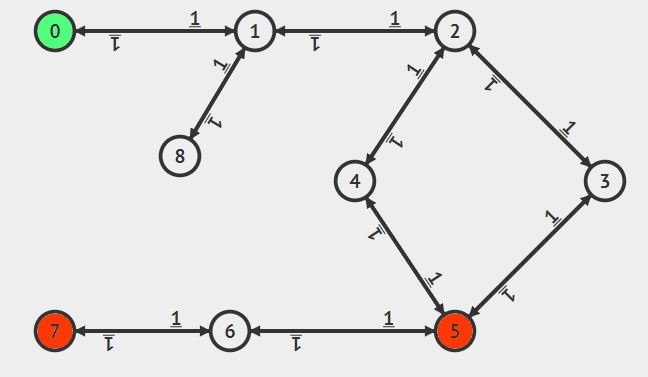
\includegraphics[height=0.4\textheight, scale=0.2, keepaspectratio]{img/alg_map_man/store_graph.JPG}
	\caption{MAP: Map of the Store}
 	\label{storeGraph}
\end{figure}
\begin{figure}[H]
\centering
	\centering
  	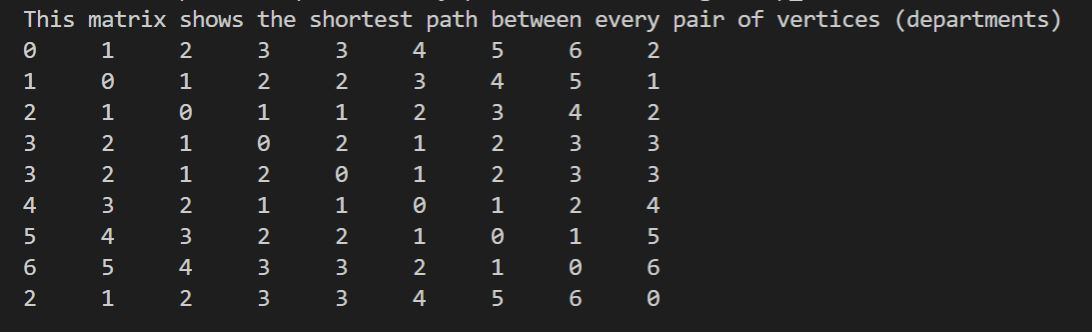
\includegraphics[height=0.2\textheight, scale=0.1, keepaspectratio]{img/alg_map_man/warshall_matr.JPG}
	\caption{SP: Shortest path between each pair of nodes in MAP}
 	\label{warshall}
\end{figure}
\begin{figure}[H]
\centering
	\centering
  	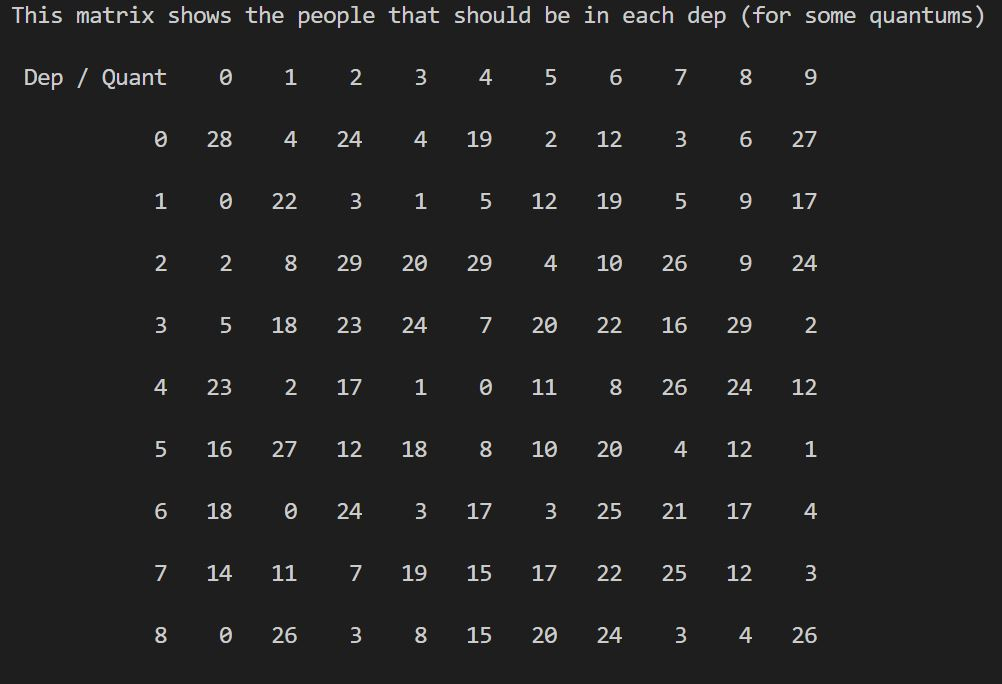
\includegraphics[height=0.4\textheight, scale=0.2, keepaspectratio]{img/alg_map_man/dep_quant_mat.JPG}
	\caption{QD: Estimated people in a specific department in a specific quantum}
 	\label{qd}
\end{figure}

Step for the algorithm:
\begin{enumerate}
    \item Each quantum has been defined to be 5 minutes-long, and that the time 8:00 is mapped to quantum 0.Thus this Visit lasts 8 quantums, from the $0^{th}$ to the $7th$. Since the Visit has only two departments, to each one of them will be assigned 8/2 = 4 quantums.
    \item We choose the entrance and exit dep. Since there is only one entrance department, 0 is selected. We have two exits. We select the exit which has the least amount of people at quantum 7 (from figure [\ref{qd}]), and it is 5 with 4 people.
    \item We create a graph with only the departments selected by the Customer and the added entrance and exit as nodes. The graph is complete and each arc has a weight equal to the shortest path from one node to another in MAP (we use the pre-computed SP (figure \ref{warshall}) to speed up the process). (figure [\ref{graphForTSP}])
    \item We add an extra node which is connected to the entrance node and the exit node with arcs of weight very small (possibly 0) and we will call this node S. Now, the problem of finding the shortest path from route to entrance to exit can be reduced to a TSP problem. (figure [\ref{graphForTSP}])
    \begin{figure}[H]
    \centering
    	\centering
      	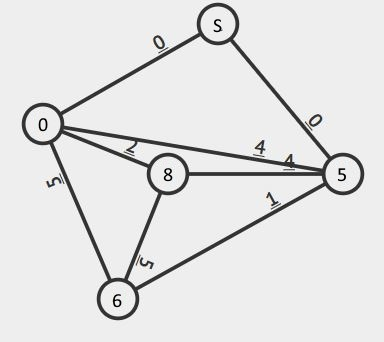
\includegraphics[height=0.4\textheight, scale=0.2, keepaspectratio]{img/alg_map_man/graph_for_tsp2.JPG}
    	\caption{Preparing graph for TSP}
     	\label{graphForTSP}
    \end{figure}
    \item In this example we just use the approximation of TSP using MST and we compute the MST using Prim's algorithm (Figure [\ref{mst}]).\newline
    If we read the nodes of the constructed MST in preorder-walk adding 0 at the end, we get: 0 - S - 5 - 6 - 8 - 0. It's length is = 0 + 2 + 5 + 1 + 0 = 8. We can see that if we traverse the path backwards and we delete the first two nodes, we obtain the path: 0 - 8 - 6 - 5. Which is what we were looking for. (and it still has length 8)
    \begin{figure}[H]
    \centering
    	\centering
      	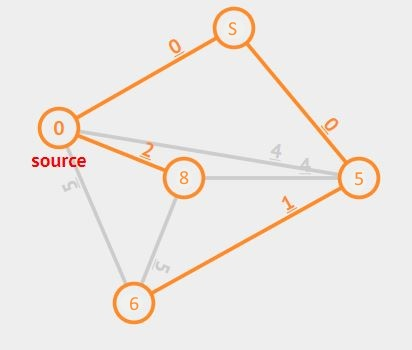
\includegraphics[height=0.4\textheight, scale=0.2, keepaspectratio]{img/alg_map_man/mst2.JPG}
    	\caption{MST of graph in figure \ref{graphForTSP}}
     	\label{mst}
    \end{figure}
    \item Since in this example we compute a single path, we would not need to check P[i, f]d in each department, but to better understand the algorithm, we now compute MAXP anyway. Since the first real department to be visited is 8, to it will be assigned the quantums from 0 to 3 included, and to department 5 will be assigned the quantums from 4 to 7 included \newline
    $MAXP = \max{\floor{(0 + 26 + 3 + 8)/4}, \floor{(8 + 10 + 20 + 4)/4}} = \max{9, 10} = 10$.
    \item Given the best path, we remove node S from it, and we save the result in VCQ, setting IsMapped to true and updating QD accordigly: (we add 1 to: (0, 0), (5, 7), (8, from 0 to 3 included), (6, from 4 to 7 included)).
    \item From this path we can easily compute the real path on MAP using, for example, Dijkstra algorithm to between each pair of ordered nodes. (figure \ref{afterDij})
    \begin{figure}[H]
    \centering
    	\centering
      	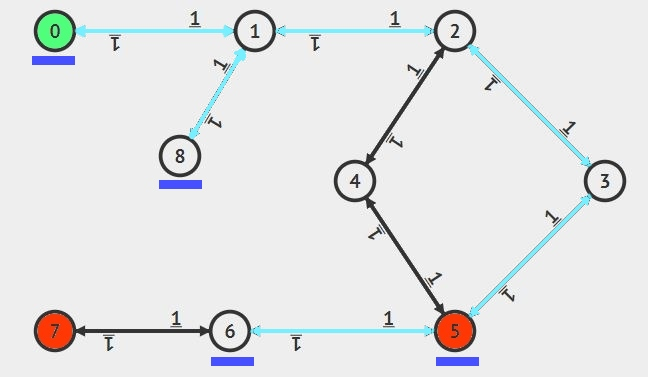
\includegraphics[height=0.4\textheight, scale=0.2, keepaspectratio]{img/alg_map_man/store_graph_PATH.JPG}
    	\caption{Created map for the Visit}
     	\label{afterDij}
    \end{figure}
\end{enumerate}

\vspace{0.4em}
\textbf{Final Considerations on the Map Creation} \newline
\vspace{0.4em}

The approach used does not give as an optimal solution neither for the shortest path problem nor for the overcrowding one. It tries to give a sub-optimal problems. Since the overcrowding that we mostly want to avoid is the one at the entrances and at the exits (so that a minor number of queues is generated), both entrance and exit are computed looking only at the estimated amount of people that should use them at a given quantum. \newline
To achieve the optimal solution for the shortest path problem, we should have used a brute-foce algorithm with time complexity O(n!), which would constraint the possible number of departments that the user can select to 9-10. Since the system could be used by large Stores, we thought, that we should give a more efficient solution. It is though possible to apply different algorithms, basing the choice on the number of selected departments in the Visit (thus, it is possible to solve TSP chosing a different algorithm from the one in the example).


\newpage
\section{User Interface Design}

\subsection{Mockup}
\begin{figure}[h!]
\centering
\begin{subfigure}
	\centering
  	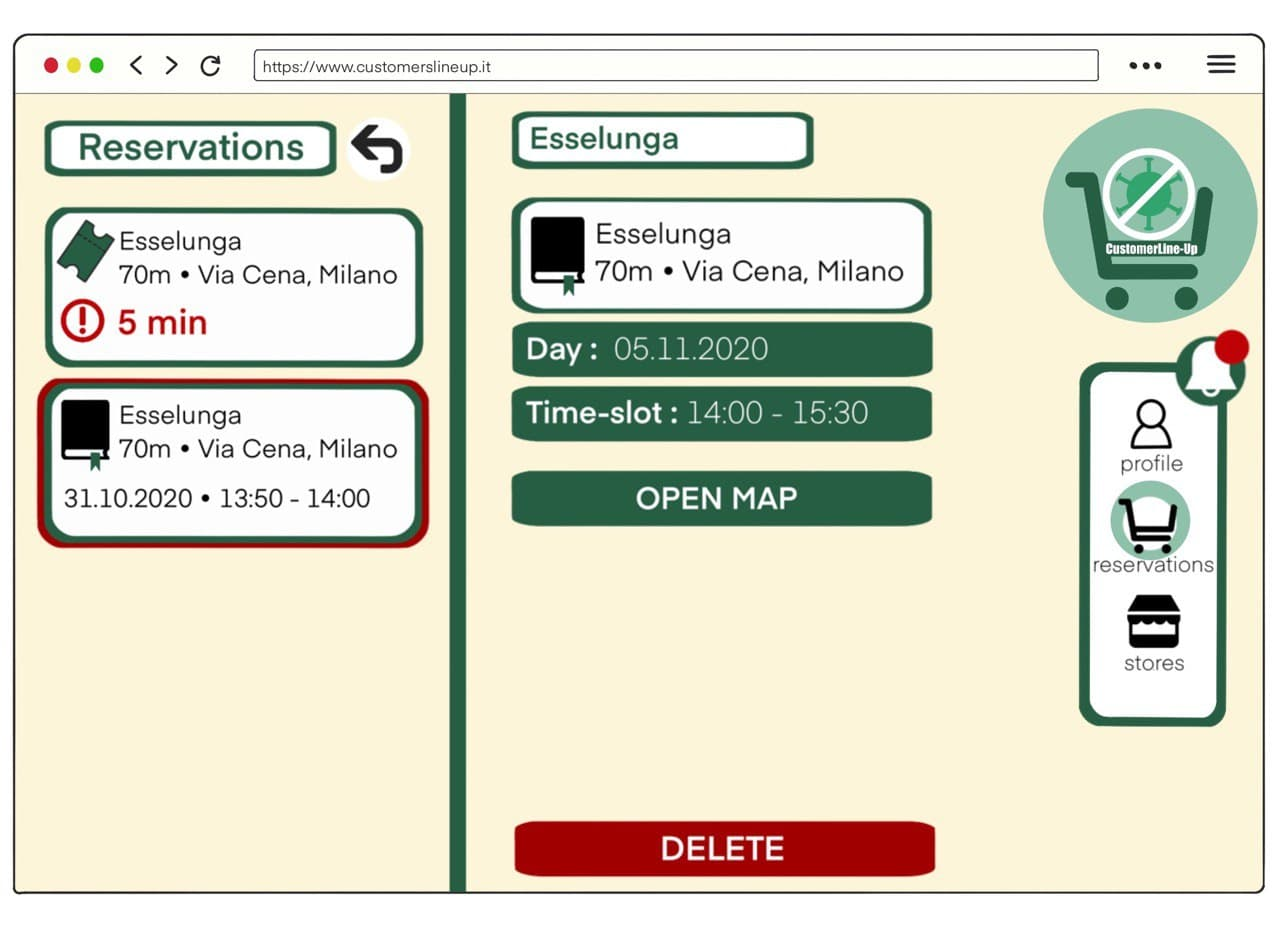
\includegraphics[height=0.4\textheight, scale=0.2, keepaspectratio]{img/customer_interface.jpg} 
 \end{subfigure}
 \begin{subfigure}
	\centering
  	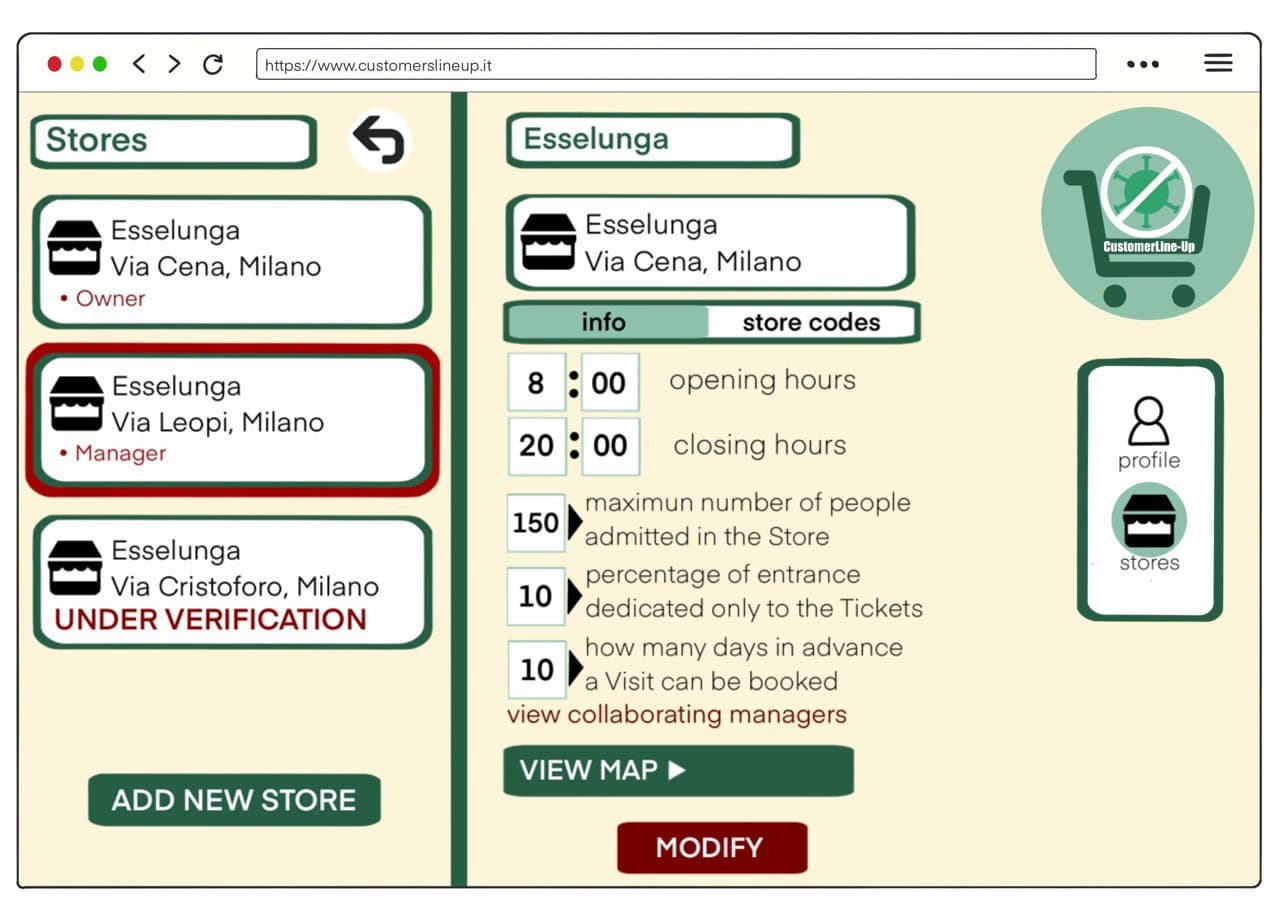
\includegraphics[height=0.4\textheight, scale=0.2, keepaspectratio]{img/manager_interface.jpg}
 \end{subfigure}
	\caption{Web page graphics.}
 	\label{web_graphics}
\end{figure}

\subsection{User Experience Diagram}
To better define the most important Users action within the application, we reported in Figure \ref{customer_experience} and in Figure \ref{manager_experience} two User Experience diagrams (UX), one for the Customer and one for the Manager. User Experience diagrams are diagrams that display the complete path a User takes when using a product, it refers to the functions and respective interfaces of the application.
\begin{figure}[h!]
\centering
	\centering
  	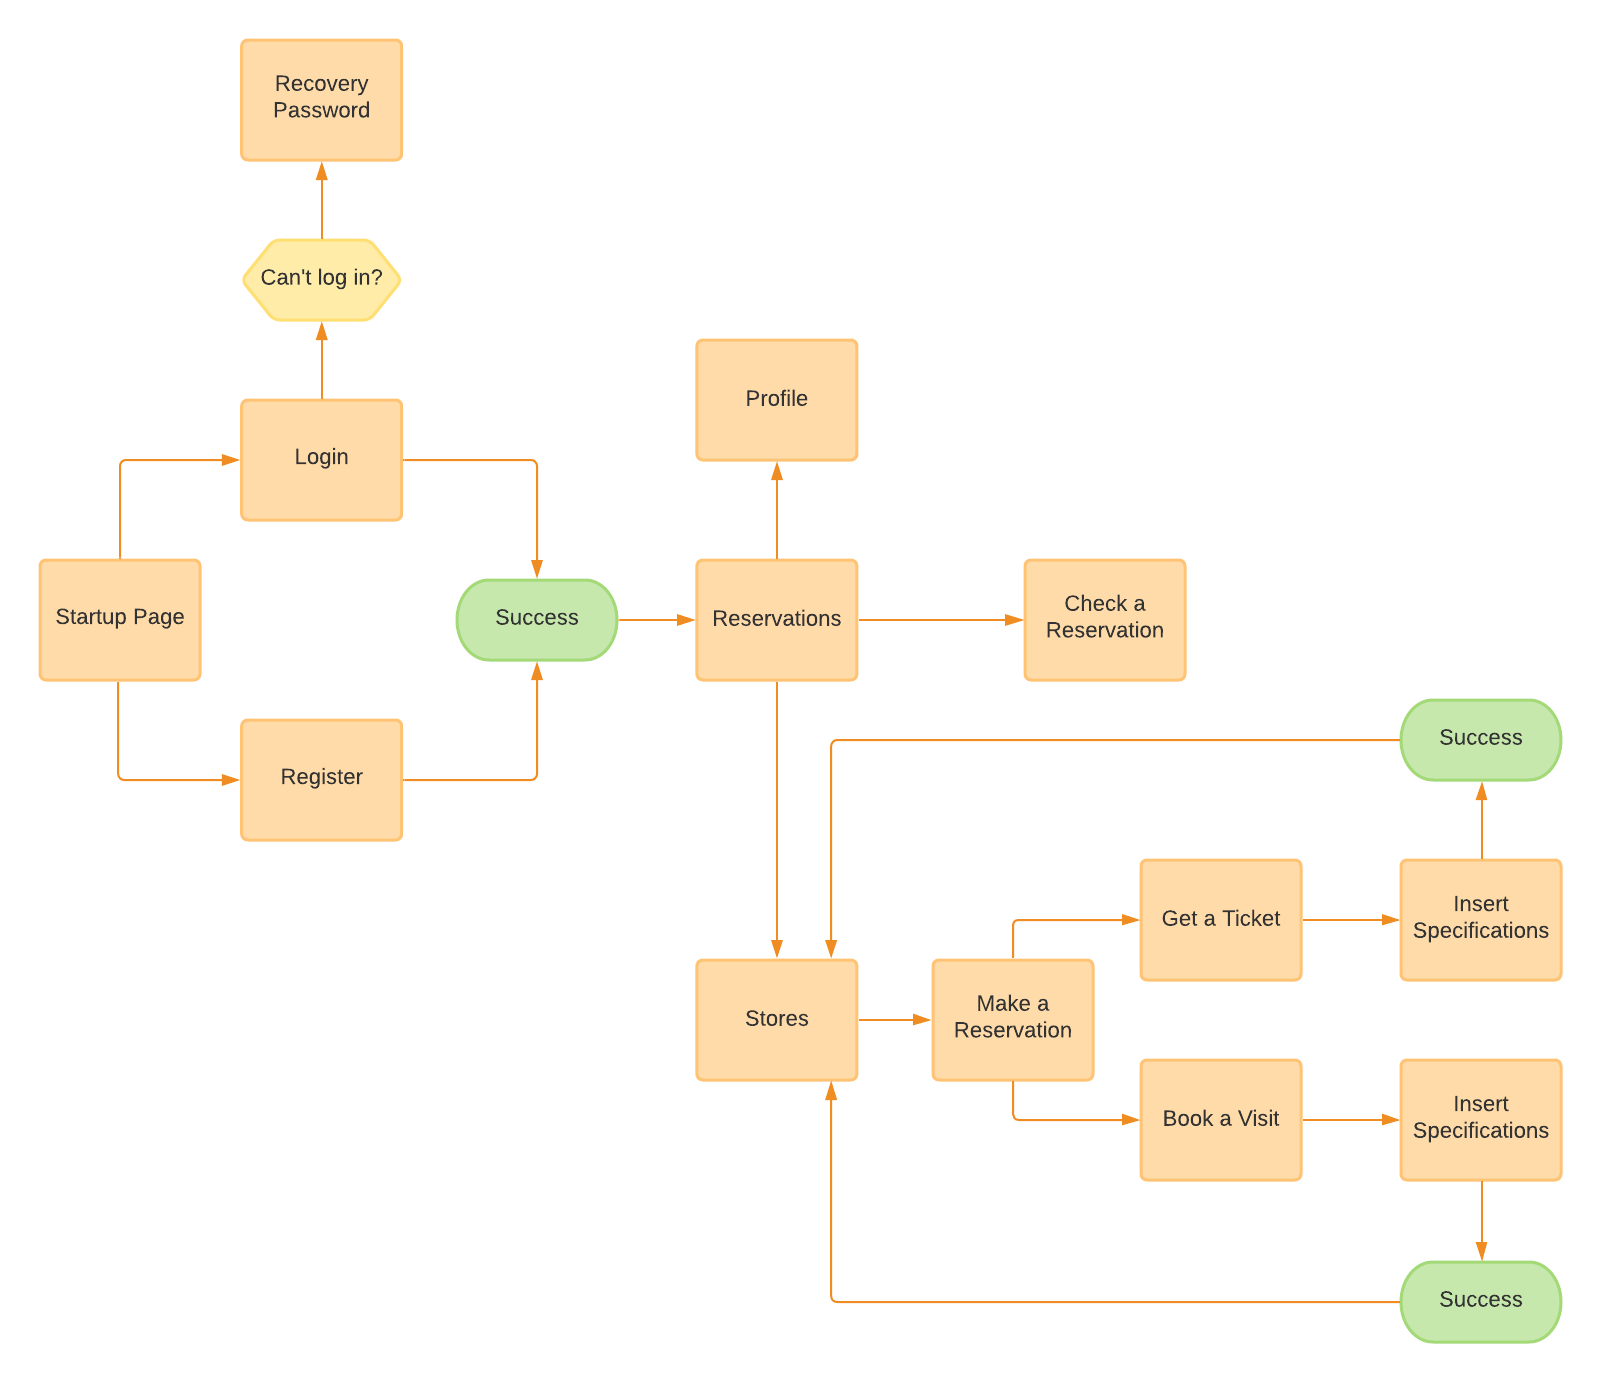
\includegraphics[height=0.5\textheight, scale=0.2, keepaspectratio]{img/customer_experience.png} 
  	\caption{UX flow of a Customer User.}
 	\label{customer_experience}
\end{figure}
\newpage
 \begin{figure}[h!]
	\centering
  	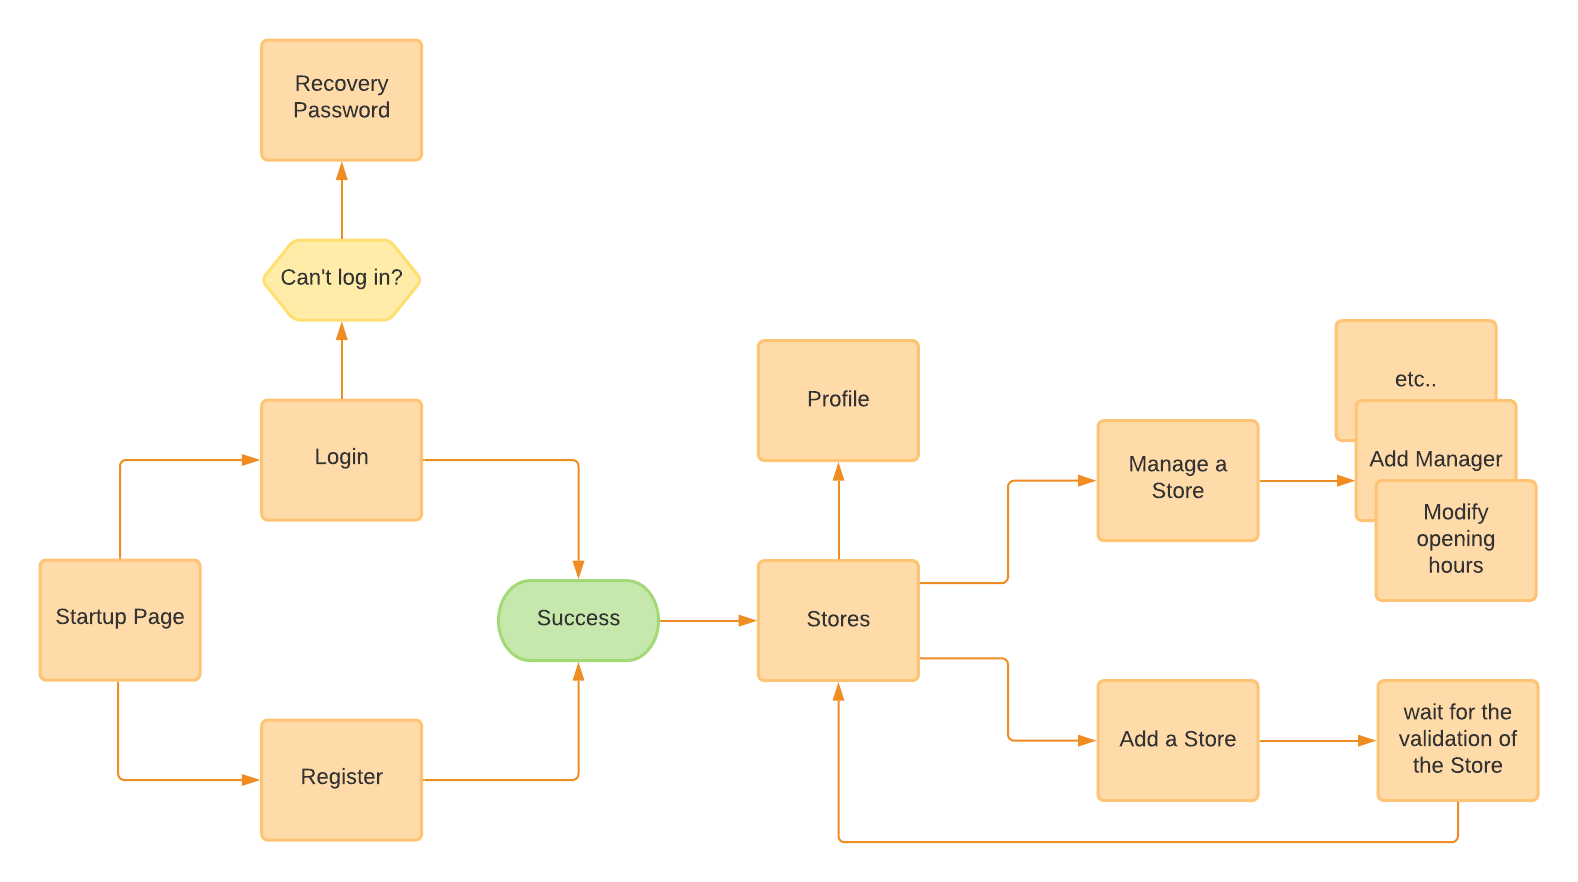
\includegraphics[height=0.35\textheight, scale=0.2, keepaspectratio]{img/manager_experience.png}
	\caption{UX flow of a Manager User.}
 	\label{manager_experience}
\end{figure}

\end{document}
